% #########################################################################
% #                       EXPLORACIÓN Y ANÁLISIS DE DATOS                 #
% #########################################################################

% Definición de nombres
\newcommand{\estudiante}{García Justel, Alan}
\newcommand{\titulo}{MÁSTER EN INGENIERÍA COMPUTACIONAL Y SISTEMAS INTELIGENTES}
\newcommand{\asignatura}{EXPLORACIÓN Y ANÁLISIS DE DATOS}
\newcommand{\portada}{common/no_signal.png}
\newcommand{\colorportada}{title_green}
\newcommand{\curso}{2024-2025}


% Notebook
\begin{document}
\newgeometry{bottom=2cm}

\begin{titlepage}
    % Logo de la universidad
    \begin{textblock*}{\textwidth}(2cm,0.4cm)
        \begin{center}
            \begin{minipage}{0.45\textwidth}
                \centering
                
\includegraphics[width=\textwidth]{common/Logo_EHU.jpg}
            \end{minipage}\hfill
            \begin{minipage}{0.45\textwidth}
                \centering
                
\includegraphics[width=0.8\textwidth]{common/Logo_KISA.png} 
            \end{minipage}
        \end{center}
    \end{textblock*}
    
    % Franja de color
    \begin{tikzpicture}[remember picture, overlay]
        \fill[\colorportada] (current page.north west) ++ (0,-3.01cm) rectangle (\paperwidth,-3cm);
    \end{tikzpicture}
    
    \begin{textblock*}{\paperwidth}(\dimexpr\parindent+\oddsidemargin+3em\relax,3.5cm)
        \begin{minipage}{\dimexpr\linewidth-7.5cm\relax}
            \color{white}
            \noindent\rule{\linewidth}{0cm}
            \textsf{ {\large \titulo}}
            \newline
            \newline \newline
            \textsf{\textbf{ {\Huge APUNTES DE ASIGNATURA }}}
        \end{minipage}
    \end{textblock*}
    
    % Nombre asignatura
    \vspace*{3.5cm}
    \begin{minipage}{\linewidth}
        \setlength{\baselineskip}{1.7\baselineskip}
        \centering
        \textsf{ \textbf{ {\LARGE \asignatura }}}
    \end{minipage}

    % Foto de portada
    \vspace*{0.5cm}
    \begin{figure}[H]
        \centering
        \includegraphics[width=10cm, height=8cm]{\portada}
    \end{figure}

    
    
    % Estudiante
    \vspace{0.2cm}
    \noindent {\footnotesize \textbf{Estudiante:} \estudiante}
    \newline
    \noindent\makebox[\linewidth]{\rule{\textwidth}{0.4pt}} % Línea horizontal

    % Curso y Fecha
    \vspace{0.1cm}    
    \noindent {\footnotesize \textbf{Curso: } \curso \hfill \textbf{Fecha:} \today }
\end{titlepage}

\restoregeometry
\setcounter{figure}{0} % Incluimos el título
\newpage
% Índices
% \tableofcontents\thispagestyle{empty} %\newpage
% \listoffigures\thispagestyle{empty}   %\newpage
% \listoftables\thispagestyle{empty}    %\newpage

\section{Visualización de Datos y Estadísticos}
Se utiliza la notación nxp individuos por filas y atributos por columnas. Cuando nos refiramos al individuo siempre en forma de vector columna.
\ex{Media en variables binarias}{
    \[
        X = \text{'Tiene una anomalía'}
    \]
    \[
        X = 
        \begin{pmatrix}
            0 \\
            1 \\
            0 \\
            0 \\
            0
        \end{pmatrix}
        \quad \mean{X} = \frac{1}{5} = 0.2
    \]
    Nos devuelve la frecuencia del 1 (probabilidad de que ocurra 1)
}

Con una matriz de correlaciones solo podemos capturar o identificar relaciones lineales. Ejemplo de la correlación cuadrática.



\subsection{Exploración Gráfica con R}
Existen dos librerías base para graficar con R. Por un lado contamos con las funciones básicas provistas por la librería estándar de R con las que podemos realizar exploraciones rápidas y sencillas y por otro lado contamos con la librería ggplot2 para realizar gráficas más avanzadas.

Por otra parte, R tiene ya muchos colores predefinidos. Algunos ya los has utilizado pero a continuación tienes más. En R base hay varias paletas de colores: colors, rainbow. . . pero además, hay diversos paquetes para manejar colores, por ejemplo RColorBrewer, que permiten marcar contrastes, o graduaciones en la escala de colores.


pch values -> Valor para los plots que indican el icono del punto a plotear (0: 25)
\newpage
\qs{Obtén una serie de gráficos a partir de estos datos}{
    {\tiny
    
    Entre los estudios que realiza periódicamente EUSTAT está el del uso del tiempo que hacemos. En este apartado trabajaremos con datos (TiempoActividad.csv) derivados de este tiempo. Las variables que tenemos son:
    \begin{itemize}
        \item SEXO
        \item EDAD (categorizada)
        \item HORARIO (0: Sin ocupación; 1: Jornada sin trabajo; 2: Trabajo sin horario; 3: Horario de mañana o normal; 4: Horario de tarde; 5: Horario de noche)
        \item JORNADA (SinOcup: Sin ocupación; Normal: Día de trabajo normal; MediaJ: Día de media jornada laboral; DescansoNOTRAB: Día de descanso festivo no trabajado; DescansoSITRAB: Día de descanso o festivo trabajado; BajaEnf : Día de baja por enfermedad; Festivo: Día de vacaciones; Otros: Otros casos)
        \item TiempoLAB (Duración de la actividad a un dígito <<Trabajo profesional y tiempo de formación>> (segundos))
        \item TiempoCUIDADO (Duración de la actividad a un dígito <<Cuidados a las personas del hogar>> (segundos))
        \item DIASEMANA (1: Lunes; — 7: Domingo)
    \end{itemize}
    }
}

\sol 
\begin{figure}[H]
    \centering
    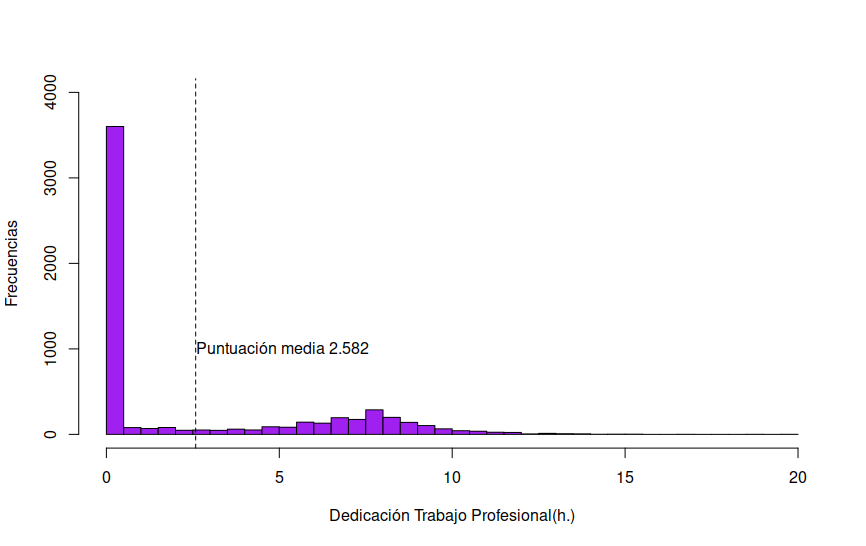
\includegraphics[width=0.6\linewidth]{EAD/images/Ejercicio_T1_E01_01.png}
    \vspace{0.5cm}
    \begin{minipage}{0.49\textwidth}
        \centering
        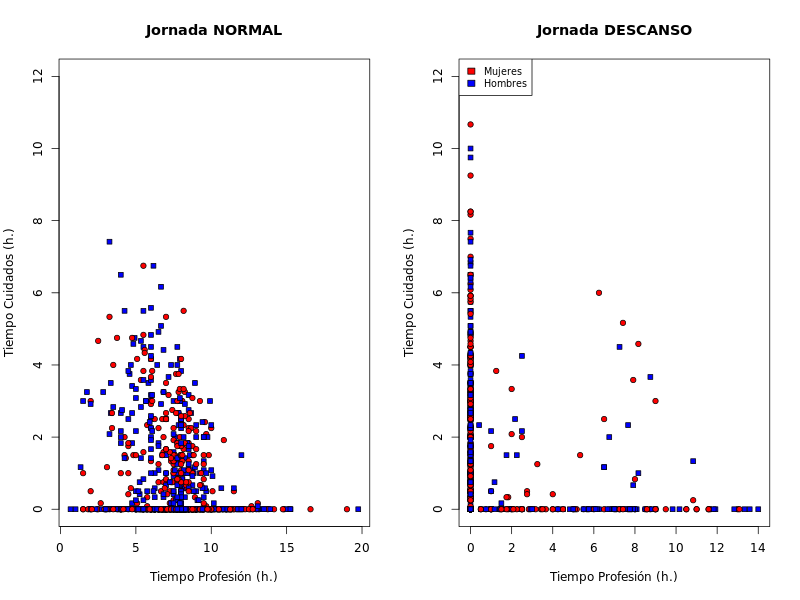
\includegraphics[width=0.7\linewidth]{EAD/images/Ejercicio_T1_E01_02.png}
    \end{minipage}
    \hfill
    \begin{minipage}{0.49\textwidth}
        \centering
        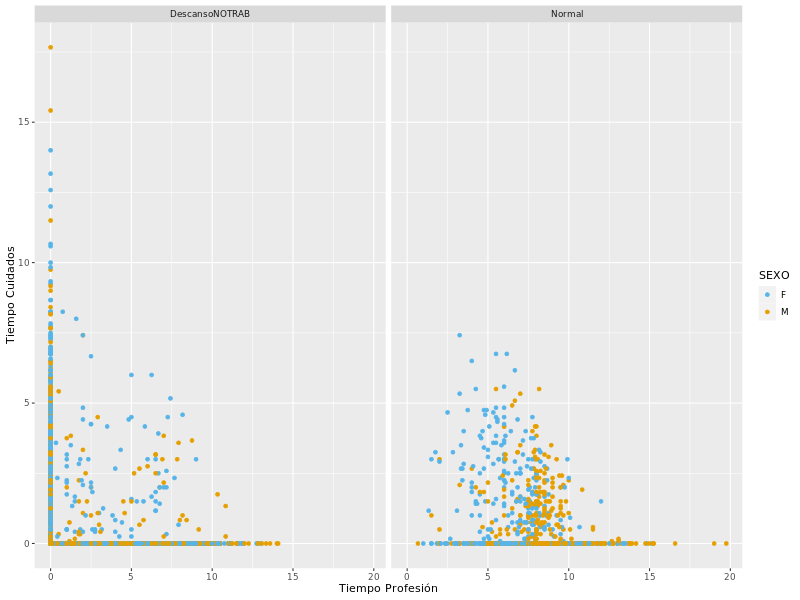
\includegraphics[width=0.7\linewidth]{EAD/images/Ejercicio_T1_E01_03.png}
    \end{minipage}
    
    \caption{Gráficas resultado del ejercicio. El código se puede encontrar en la carpeta de ejercicios}
\end{figure}



\section{Repaso Álgebra}
El producto escalar es la sombra de un vector sobre otro

Si centramos dos veces tenemos la matriz de varianzas covarianzas

Vectores propios y valores propios



\end{document}